\documentclass{beamer}

\usepackage{graphicx}
\usepackage{hyperref}
\usepackage{tikz}
\usetikzlibrary{positioning}

\title{The Mandelbrot Set \\ Hybrid MPI/OpenMP Implementation} 
\author{Alessandro Della Siega}
\institute{University of Trieste}
\date{May 2024}

\begin{document}

\frame{\titlepage}


%%%%%%%%%%% SLIDE %%%%%%%%%%%

\begin{frame}
    \frametitle{Introduction}

    The goal is to implement and analyze a \textbf{hybrid MPI/OpenMP} implementation of the computation of the Mandelbrot set, which is defined as:
    $$
        \mathcal{M} = \{c \in \mathbb{C} : \lim_{n \to \infty} z_n < \infty \}
    $$
    where $z_{n+1} = z_n^2 + c$ and $z_0 = 0$.

    \begin{columns}
        
        \begin{column}{0.5\textwidth}
            
            \begin{figure}
                \centering
                
\includegraphics[width=0.7\textwidth]{../images/mandelbrot.png}
                \caption{Rendering of the Mandelbrot set. } 
            \end{figure}

        \end{column}
        
        \begin{column}{0.5\textwidth}
            Encoding:
            \begin{itemize}
                \item each pixel represents a complex number $c$.
                \item the color of the pixel depends on the number of iterations before $z_n$ diverges.
            \end{itemize}
        \end{column}

    \end{columns}   

\end{frame}


%%%%%%%%%%% SLIDE %%%%%%%%%%%
\begin{frame}
    \frametitle{Computational architecture}
    ORFEO cluster

    EPYC paritition

    \begin{itemize}
        \item 8 nodes
        \item 2x AMD EPYC 7742 64-Core Processor on each node
        \item 512 GB RAM
    \end{itemize}

    For our purposes we will use at most 2 nodes of the EPYC partition.
\end{frame}


%%%%%%%%%%% SLIDE %%%%%%%%%%%
\begin{frame}
    \frametitle{Parallelization strategy}
 
    \begin{columns}

        \begin{column}{0.5\textwidth}
            We adopt a sequential fashion:
            \begin{enumerate}
                \item using MPI, initialize $P$ processes 
                \item each process computes a portion of the image using $T$ OpenMP threads (loop scheduling policy is set to \texttt{dynamic})
                \item the master process uses \texttt{MPI\_Gatherv} to collect the results
            \end{enumerate}
        \end{column}

        \begin{column}{0.5\textwidth}
            \begin{figure}
                \centering
                
\includegraphics[width=0.7\textwidth]{../images/process_subdivision.png}
                \caption{Suppose to have 4 processes. Each process will compute a portion of the image.}
            \end{figure}
            Let $N = n_x \times n_y$ be the total number of pixels.
            Each process will compute approximately $N/P$ pixels.
        \end{column}

    \end{columns}

\end{frame}

%%%%%%%%%%% SLIDE %%%%%%%%%%%
\begin{frame}
    \frametitle{Experimental setup}

    \begin{columns}
        \begin{column}{0.5\textwidth}
            \center

            \textbf{MPI scaling}
            
            Set $T=1$ and vary $P = 1,2,4,8, \dots, 112, 128$

            \begin{itemize}
                \item strong scaling: $$n_x = n_y = 4096$$
                \item weak scaling: $$n_x = n_y = 1024 \times \texttt{round} \{\sqrt{P}\}$$
            \end{itemize}
        \end{column}

        \begin{column}{0.5\textwidth}
            \center
            \textbf{OpenMP scaling}
            
            Set $P=1$ and vary $T = 2,4,6,8, \dots, 62,64$
            
            \begin{itemize}
                \item strong scaling: $$n_x = n_y = 4096$$
                \item weak scaling:
                $$n_x = n_y = 1024 \times \texttt{round} \{\sqrt{T}\}$$
            \end{itemize}

        \end{column}
    
    \end{columns}

\end{frame}

%%%%%%%%%%% SLIDE %%%%%%%%%%%
\begin{frame}
    \frametitle{Other parameters}
        \begin{itemize}
            \item For MPI, we set \texttt{--map-by core} and \texttt{--bind-to socket}
            \item For OpenMP, we set \texttt{OMP\_PLACES=cores} and no binding policy.
        \end{itemize}
\end{frame}

%%%%%%%%%%% SLIDE %%%%%%%%%%%
\begin{frame}
    \frametitle{MPI \textbf{strong} scaling results}
    \begin{figure}
        \centering
        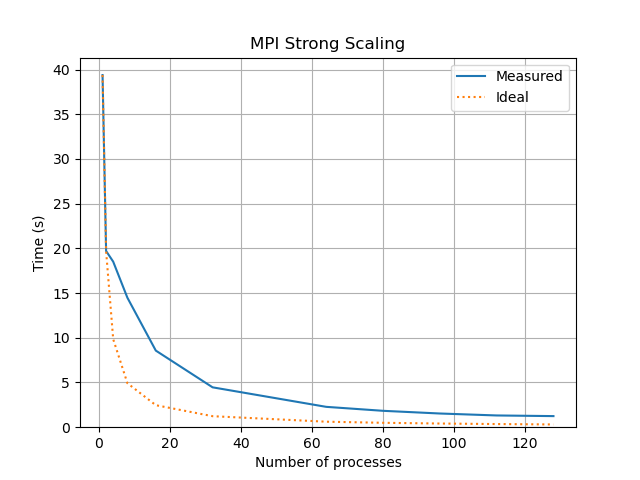
\includegraphics[width=0.5\textwidth]{../images/mpi_strong_scaling.png}
        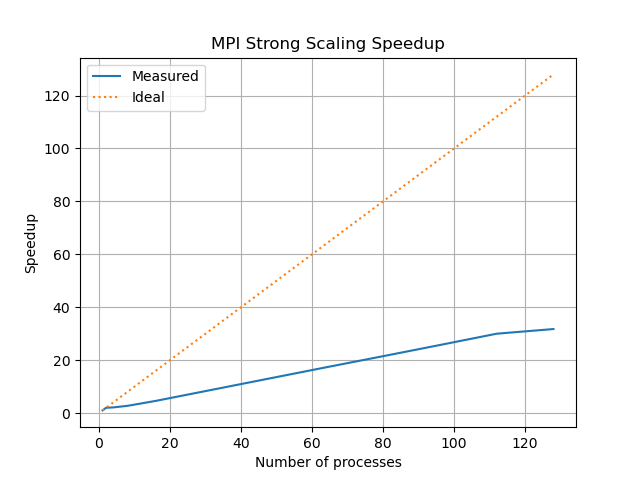
\includegraphics[width=0.5\textwidth]{../images/mpi_strong_scaling_speedup.png}
        \caption{MPI strong scaling results.}
    \end{figure}
\end{frame}


%%%%%%%%%%% SLIDE %%%%%%%%%%%
\begin{frame}
    \frametitle{MPI \textbf{weak} scaling results}
    \begin{figure}
        \centering
        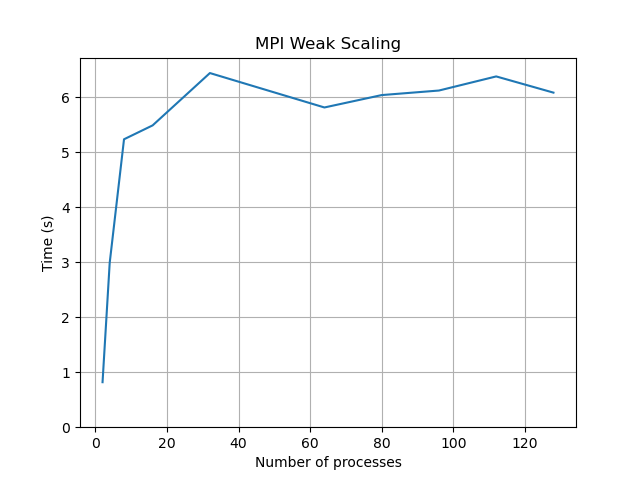
\includegraphics[width=0.5\textwidth]{../images/mpi_weak_scaling.png}
        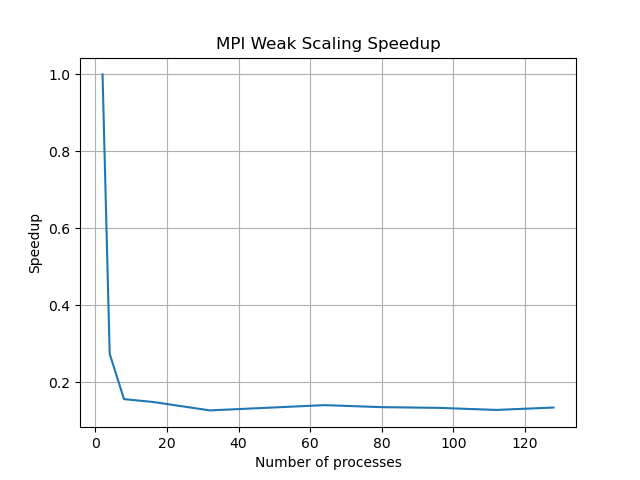
\includegraphics[width=0.5\textwidth]{../images/mpi_weak_scaling_speedup.png}
        \caption{MPI weak scaling results.}
    \end{figure}
\end{frame}


%%%%%%%%%%% SLIDE %%%%%%%%%%%
\begin{frame}
    \frametitle{OpenMP \textbf{strong} scaling results}
    \begin{figure}
        \centering
        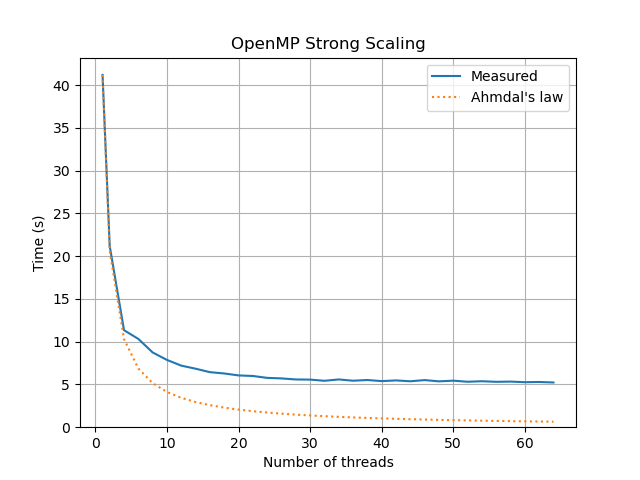
\includegraphics[width=0.5\textwidth]{../images/omp_strong_scaling.png}
        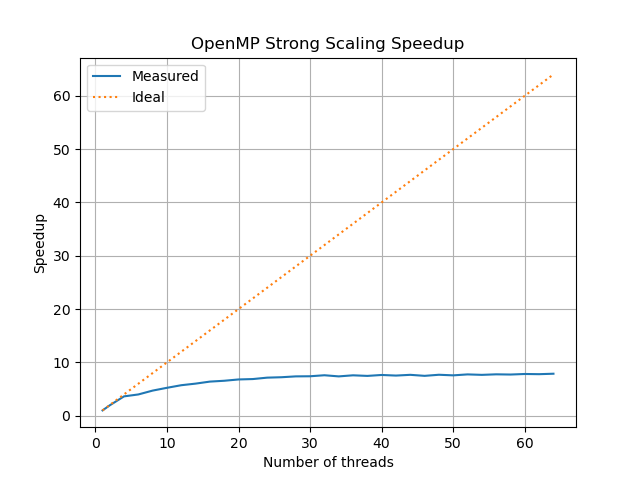
\includegraphics[width=0.5\textwidth]{../images/omp_strong_scaling_speedup.png}
        \caption{OMP strong scaling results.}
    \end{figure}
\end{frame}

%%%%%%%%%%% SLIDE %%%%%%%%%%%
\begin{frame}
    \frametitle{OpenMP \textbf{weak} scaling results}
    \begin{figure}
        \centering
        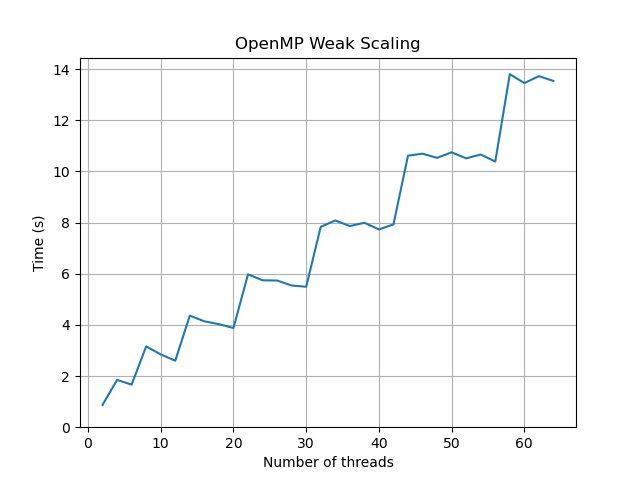
\includegraphics[width=0.5\textwidth]{../images/omp_weak_scaling.png}
        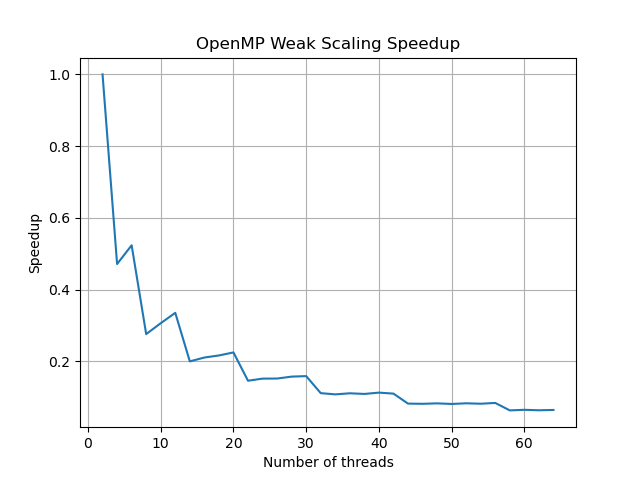
\includegraphics[width=0.5\textwidth]{../images/omp_weak_scaling_speedup.png}
        \caption{OpenMP weak scaling results.}
    \end{figure}
\end{frame}

%%%%%%%%%%% SLIDE %%%%%%%%%%%
\begin{frame}
    \frametitle{Conclusions}
    \begin{itemize}
        \item MPI scaling shows an expected behavior for both strong and weak scaling
        \item OpenMP strong scaling shows that we reach a bottleneck
    \end{itemize}
     
    OpenMP issues:
    \begin{itemize}
        \item load imbalance
        \item false sharing
    \end{itemize}

    Improvements:
    \begin{itemize}
        \item smarter load balancing strategy
        \item exploit symmetries
        \item exploit compiler optimizations
    \end{itemize}

\end{frame}



\end{document}